\documentclass[11pt,a4paper]{article}

\usepackage[utf8]{inputenc}
\usepackage[T1]{fontenc}
\usepackage[spanish]{babel}
\usepackage{geometry}
\usepackage{graphicx}
\usepackage{float}
\usepackage{booktabs}
\usepackage{array}
\usepackage{longtable}
\usepackage{caption}
\usepackage[table]{xcolor}
\usepackage{hyperref}
\usepackage{listings}
\usepackage{amsmath}
\usepackage{needspace}
\usepackage{newtxtext}
\usepackage{newtxmath}
\usepackage[final]{microtype}

\geometry{a4paper, margin=2.3cm}
\input{glyphtounicode}
\pdfgentounicode=1
\hypersetup{
  hidelinks,
  pdftitle={Determinantes de los precios de la vivienda en Alcobendas},
  pdfauthor={Alejandro Rodríguez, Gaspar Muñoz, Alonso Castro y Jaime Blanco}
}
\setlength{\parindent}{0pt}
\setlength{\parskip}{0.55em}
\setlength{\textfloatsep}{14pt plus 2pt minus 3pt}
\setlength{\floatsep}{12pt plus 2pt minus 2pt}
\setlength{\intextsep}{12pt plus 2pt minus 2pt}
\setlength{\belowcaptionskip}{2pt}
\setlength{\tabcolsep}{7pt}
\renewcommand{\arraystretch}{1.16}
\emergencystretch=1.5em
\addto\captionsspanish{%
  \renewcommand{\figurename}{Gráfico}%
  \renewcommand{\tablename}{Tabla}%
}
\captionsetup{labelsep=period, font=small, labelfont=bf, skip=8pt}
\captionsetup[table]{skip=7pt}
\captionsetup[figure]{skip=9pt}

\definecolor{accent}{RGB}{29,52,84}
\definecolor{textgray}{RGB}{72,76,82}
\definecolor{softgray}{RGB}{245,246,248}
\definecolor{tablehead}{RGB}{236,239,243}
\definecolor{tablerow}{RGB}{249,250,251}

\lstdefinestyle{rstyle}{
  language=R,
  inputencoding=utf8,
  basicstyle=\ttfamily\footnotesize,
  keywordstyle=\color{blue!60!black},
  commentstyle=\color{green!35!black},
  stringstyle=\color{red!45!black},
  numbers=left,
  numberstyle=\tiny\color{gray},
  stepnumber=1,
  numbersep=8pt,
  showstringspaces=false,
  breaklines=true,
  frame=single,
  rulecolor=\color{black!20},
  columns=fullflexible
}

\title{\textbf{Determinantes de los precios de la vivienda en Alcobendas}\\[0.4em]\large Informe final de Econometría}
\author{Alejandro Rodríguez \and Gaspar Muñoz \and Alonso Castro \and Jaime Blanco}
\date{6 de mayo de 2026}

\begin{document}

\begin{titlepage}
  \pagenumbering{gobble}
  \thispagestyle{empty}
  \color{textgray}
  \vspace*{-1.05cm}
  \noindent\hspace*{-0.12cm}
\includegraphics[width=0.305\textwidth]{logo_cunef_eps.jpg}\par
  \vspace{3.35cm}
  {\color{accent}\rule{\textwidth}{1.3pt}\par}
  \vspace{1.15cm}
  \begin{center}
    {\fontsize{23}{29}\selectfont\bfseries\color{black} Determinantes de los precios de la vivienda en Alcobendas\par}
    \vspace{0.5cm}
    {\Large\color{accent} Proyecto de Econometría\par}
    \vspace{0.85cm}
    {\normalsize\bfseries Autores\par}
    \vspace{0.2cm}
    {\large Alejandro Rodríguez, Gaspar Muñoz,\par}
    {\large Alonso Castro y Jaime Blanco\par}
  \end{center}
  \vspace{1.15cm}
  \noindent\colorbox{softgray}{%
    \parbox{\dimexpr\textwidth-2\fboxsep\relax}{%
      \vspace{0.35cm}
      \begin{tabular}{@{}>{\bfseries}p{4.3cm}p{8.6cm}@{}}
        Asignatura: & Econometría \\
        Curso académico: & 2025/2026 \\
        Municipio asignado: & Alcobendas \\
        Fecha: & 6 de mayo de 2026 \\
      \end{tabular}
      \vspace{0.35cm}
    }%
  }
  \vfill
  {\color{accent}\rule{\textwidth}{0.7pt}\par}
  \vspace{0.35cm}
  {\footnotesize Base de datos empleada: \texttt{idealista\_es\_sale\_homes\_madrid\_pages84\_2025-07-15.csv}\par}
\end{titlepage}

\pagenumbering{arabic}
\tableofcontents
\clearpage

\Needspace{10\baselineskip}
\section{Datos y filtrado}

El análisis se realiza sobre el fichero de Idealista facilitado en el enunciado, con 4.200 observaciones y 49 variables. Siguiendo exactamente la pauta del profesor, se ha filtrado la base para conservar solo los anuncios con \texttt{\detokenize{municipality == "Alcobendas"}} y \texttt{\detokenize{operation == "sale"}}, y después se han retenido únicamente las variables \texttt{price}, \texttt{propertyType}, \texttt{size}, \texttt{rooms}, \texttt{bathrooms} y \texttt{status}. La limpieza básica consiste en eliminar observaciones con valores perdidos en esas columnas y construir las variables derivadas \texttt{log\_price} y \texttt{log\_size}.

La muestra final queda reducida a 19 anuncios válidos. Es una muestra pequeña para un análisis hedónico, por lo que conviene interpretar con prudencia tanto los contrastes de significación como los coeficientes de las variables categóricas. Aun así, el ejercicio sigue siendo útil como aproximación aplicada a Alcobendas y permite identificar qué características parecen más vinculadas al precio anunciado.

El análisis se trata como un corte transversal de anuncios inmobiliarios: no se explota una dimensión temporal ni se introducen rezagos, tendencias o estacionalidad.

\begin{table}[H]
\centering
\caption{Composición de la muestra tras el filtrado y la limpieza}
\label{tab:muestra}
\small
\rowcolors{2}{tablerow}{white}
\begin{tabular}{p{8.2cm}r}
\toprule
\rowcolor{tablehead}
Concepto & Observaciones \\
\midrule
Base completa de anuncios & 4.200 \\
Variables originales del fichero & 49 \\
Municipio analizado & Alcobendas \\
Condición de filtrado & venta (\texttt{sale}) \\
Muestra final tras limpieza & 19 \\
Valores perdidos en las variables seleccionadas & 0 \\
\addlinespace
Tipo de propiedad: \texttt{flat} & 15 \\
Tipo de propiedad: \texttt{duplex} & 2 \\
Tipo de propiedad: \texttt{penthouse} & 2 \\
\addlinespace
Estado: \texttt{good} & 16 \\
Estado: \texttt{newdevelopment} & 3 \\
\bottomrule
\end{tabular}
\end{table}

La Tabla \ref{tab:muestra} deja claro que la mayor parte de la muestra está formada por pisos en buen estado. Esa concentración ayuda a entender por qué algunas variables ficticias (dummies) tienen poca potencia estadística: los grupos minoritarios apenas cuentan con dos o tres observaciones.

\Needspace{9\baselineskip}
\section{Descripción de la muestra}

La muestra representa un segmento relativamente homogéneo del mercado de venta residencial de Alcobendas. Predominan los pisos frente a otras tipologías y, además, la mayor parte de los anuncios se concentra en inmuebles clasificados como \texttt{good}. Esto sugiere que la heterogeneidad observable por tipo y estado existe, pero es limitada dentro de la submuestra disponible.

Desde el punto de vista sustantivo, esta composición favorece que el tamaño tenga un papel central en la explicación del precio: cuando hay poca variación en variables cualitativas, es habitual que los metros cuadrados recojan buena parte de las diferencias de valor entre anuncios.

\Needspace{10\baselineskip}
\section{Descriptivos}

La Tabla \ref{tab:descriptivos} resume las variables cuantitativas principales. El precio medio anunciado asciende a 555.357,89 euros, con una dispersión elevada, coherente con un mercado donde conviven viviendas medias con activos claramente más caros. El tamaño medio es de 114 m\textsuperscript{2}, mientras que el inmueble tipo de la muestra tiene entre dos y tres habitaciones y algo menos de dos baños.

\begin{table}[H]
\centering
\caption{Estadísticos descriptivos de la muestra}
\label{tab:descriptivos}
\small
\rowcolors{2}{tablerow}{white}
\begin{tabular}{lrrrr}
\toprule
\rowcolor{tablehead}
Variable & Media & Desv. típ. & Mínimo & Máximo \\
\midrule
Precio (euros) & 555.357,89 & 222.859,85 & 239.000 & 960.000 \\
Tamaño (m\textsuperscript{2}) & 114,00 & 39,24 & 61 & 176 \\
Habitaciones & 2,74 & 1,05 & 1 & 5 \\
Baños & 1,74 & 0,81 & 1 & 4 \\
\bottomrule
\end{tabular}
\end{table}

\begin{figure}[H]
  \centering
  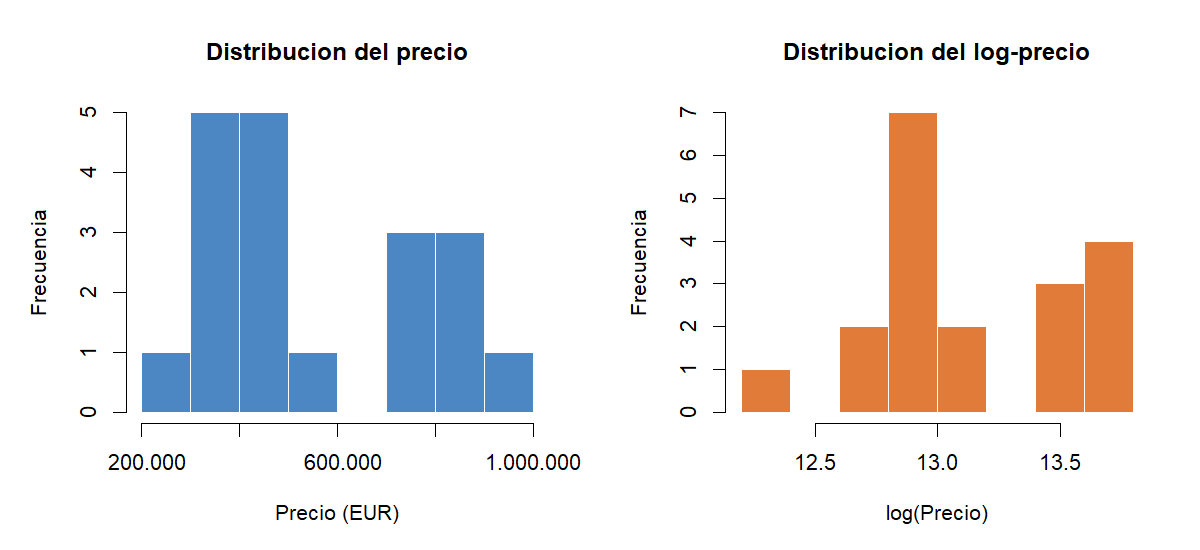
\includegraphics[width=0.9\textwidth]{../../hist_precios.png}
  \caption{Distribución del precio de los anuncios y de su transformación logarítmica en Alcobendas}
  \label{fig:hist}
\end{figure}

El Gráfico \ref{fig:hist} muestra una distribución del precio claramente asimétrica a la derecha. La transformación logarítmica suaviza esa escala, reduce el peso visual de los anuncios más caros y acerca la distribución a un patrón más regular, algo conveniente para la modelización lineal del logaritmo del precio.

\begin{figure}[H]
  \centering
  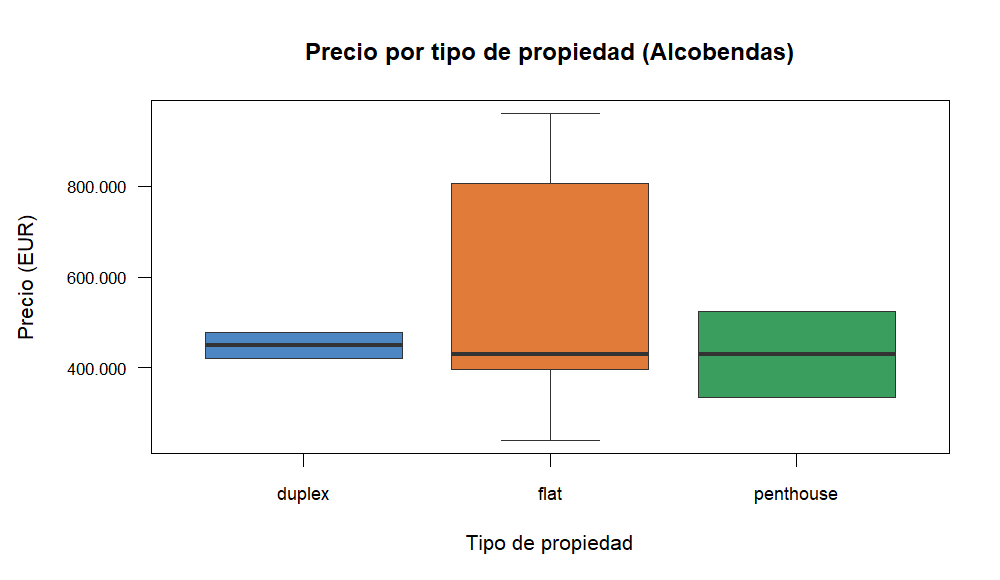
\includegraphics[width=0.78\textwidth]{../../boxplot_tipo.png}
  \caption{Distribución del precio de los anuncios por tipo de propiedad en Alcobendas}
  \label{fig:boxplot}
\end{figure}

El Gráfico \ref{fig:boxplot} sugiere diferencias de nivel entre tipos de propiedad, pero la comparación debe interpretarse con cautela porque \texttt{duplex} y \texttt{penthouse} solo cuentan con dos observaciones cada uno. Con tan poca base muestral, un valor extremo puede alterar mucho la lectura visual.

\Needspace{10\baselineskip}
\section{Regresiones simples}

Como primer paso se estiman seis regresiones univariantes. La Tabla \ref{tab:sencillas} resume los coeficientes relevantes y su capacidad explicativa. El patrón principal es claro: el tamaño explica por sí solo una parte muy importante de la variación del precio, tanto en niveles como en logaritmos. En cambio, tipo de propiedad y estado apenas aportan poder explicativo cuando se consideran de manera aislada.

\begin{table}[H]
\centering
\caption{Resumen de regresiones simples}
\label{tab:sencillas}
\footnotesize
\rowcolors{2}{tablerow}{white}
\begin{tabular}{p{3.8cm}p{4.2cm}rr}
\toprule
\rowcolor{tablehead}
Modelo & Coeficiente principal & Error estándar & $R^2$ \\
\midrule
\texttt{\detokenize{price ~ size}} & 4.949,51 (\texttt{size}) & 675,84 & 0,759 \\
\texttt{\detokenize{log_price ~ log_size}} & 0,976 (\texttt{log\_size}) & 0,138 & 0,746 \\
\texttt{\detokenize{log_price ~ rooms}} & 0,298 (\texttt{rooms}) & 0,059 & 0,602 \\
\texttt{\detokenize{log_price ~ bathrooms}} & 0,365 (\texttt{bathrooms}) & 0,082 & 0,535 \\
\texttt{\detokenize{price ~ propertyType}} & bloque \texttt{propertyType} & ver nota & 0,077 \\
\texttt{\detokenize{price ~ status}} & variables ficticias de estado & ver nota & 0,058 \\
\bottomrule
\end{tabular}
\caption*{\parbox{0.96\linewidth}{\footnotesize\textit{Nota}: en \texttt{\detokenize{price ~ propertyType}}, las dummies se estiman respecto a la categoría base \texttt{duplex}; sus errores estándar son 170.988,40 para \texttt{flat} y 227.144,81 para \texttt{penthouse}. En \texttt{\detokenize{price ~ status}}, la dummy \texttt{newdevelopment}, frente a la base \texttt{good}, tiene un error estándar de 140.054,12.}}
\end{table}

Estas regresiones se interpretan como relaciones bivariantes estimadas por MCO; por tanto, sus pendientes no deben leerse todavía como efectos \textit{ceteris paribus}. La lectura económica sigue siendo útil como primer contraste. En el modelo lineal en niveles, cada metro cuadrado adicional se asocia con aproximadamente 4.950 euros más en el precio anunciado. En el modelo log-log, la elasticidad estimada es 0,976, muy próxima a la unidad: un aumento del 1\% en el tamaño se asocia con un incremento cercano al 0,98\% en el precio. También aparecen asociaciones positivas para habitaciones y baños cuando se analizan por separado, aunque estas relaciones pueden estar capturando parcialmente el efecto del propio tamaño.

No se comparan mecánicamente los $R^2$ de modelos con distinta variable dependiente.

\Needspace{11\baselineskip}
\section{Modelo multivariante principal}

El modelo principal estimado es:
\[
\begin{aligned}
\log(price_i)=&\ \beta_0+\beta_1\log(size_i)+\beta_2 rooms_i+\beta_3 bathrooms_i\\
&+\boldsymbol{\beta}_4'\mathrm{propertyType}_i+\boldsymbol{\beta}_5'\mathrm{status}_i+u_i.
\end{aligned}
\]

La Tabla \ref{tab:principal} recoge los resultados. El ajuste es razonable para una muestra tan pequeña, con un $R^2$ de 0,794 y un $R^2$ ajustado de 0,691. El resultado más robusto es el coeficiente de \texttt{log\_size}, positivo y estadísticamente significativo al 5\%. En concreto, un aumento del 10\% en el tamaño se asocia aproximadamente con un aumento del 9,5\% en el precio, manteniendo constantes habitaciones, baños, tipo de propiedad y estado.

\begin{table}[H]
\centering
\caption{Modelo multivariante principal. Variable dependiente: \texttt{log\_price}}
\label{tab:principal}
\small
\rowcolors{2}{tablerow}{white}
\begin{tabular}{p{4.7cm}rrr}
\toprule
\rowcolor{tablehead}
Variable & Coeficiente & Error estándar & $p$-valor \\
\midrule
\texttt{log\_size} & 0,950 & 0,344 & 0,017 \\
\texttt{rooms} & -0,020 & 0,137 & 0,885 \\
\texttt{bathrooms} & 0,082 & 0,126 & 0,529 \\
\texttt{propertyType = flat} & 0,148 & 0,218 & 0,510 \\
\texttt{propertyType = penthouse} & 0,316 & 0,295 & 0,305 \\
\texttt{status = newdevelopment} & 0,012 & 0,171 & 0,943 \\
\midrule
$R^2$ & \multicolumn{3}{r}{0,794} \\
$R^2$ ajustado & \multicolumn{3}{r}{0,691} \\
\bottomrule
\end{tabular}
\end{table}

La especificación multivariante permite interpretar el coeficiente de \texttt{log\_size} en sentido \textit{ceteris paribus}, manteniendo constantes habitaciones, baños, tipo de propiedad y estado. Esta es precisamente la razón de pasar de regresiones simples a regresión múltiple, reduciendo el riesgo de sesgo por variable omitida asociado a características observables del inmueble.

Una vez que se controla por tamaño, las variables \texttt{rooms}, \texttt{bathrooms}, \texttt{propertyType} y \texttt{status} dejan de mostrar significación estadística. Esto es coherente con la idea de que una parte relevante de la información contenida en habitaciones y baños ya está recogida por los metros cuadrados. También es consistente con el pequeño tamaño muestral: con solo 19 anuncios, detectar diferencias finas entre categorías resulta difícil.

\Needspace{18\baselineskip}
\subsection{Diagnóstico básico}

\begin{figure}[H]
  \centering
  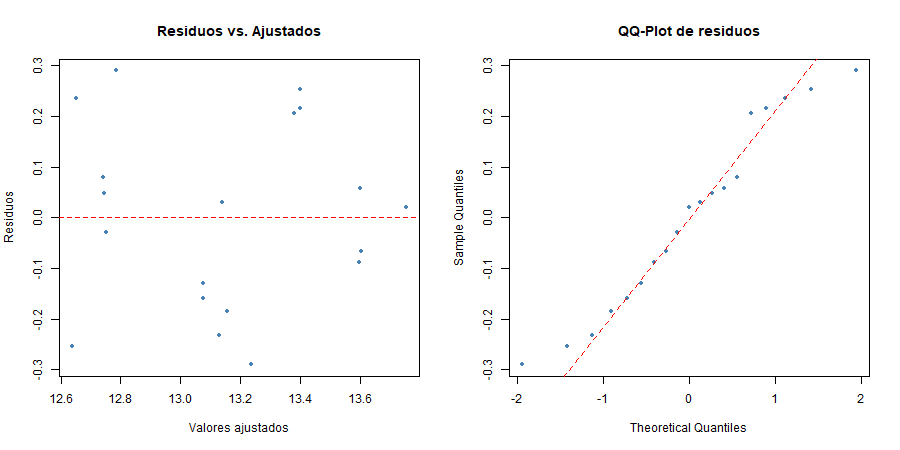
\includegraphics[width=0.86\textwidth]{../../residuos_modelo_full.png}
  \caption{Diagnóstico visual de residuos del modelo multivariante principal}
  \label{fig:residuos}
\end{figure}

El Gráfico \ref{fig:residuos} no muestra una anomalía dominante, aunque la capacidad de diagnóstico es limitada por el escaso número de observaciones. No se aprecia una pauta visual clara que obligue a replantear la especificación; por ello, esta inspección se interpreta solo como una comprobación básica y no como una validación definitiva del modelo.

\Needspace{14\baselineskip}
\section{Significación conjunta de \texttt{propertyType} mediante F-test}

Para evaluar si las dummies de tipo de propiedad añaden información de forma conjunta, se compara el modelo completo con una versión restringida que excluye \texttt{propertyType}. El contraste F arroja un $p$-valor aproximado de 0,568, por lo que no se rechaza la hipótesis nula de insignificancia conjunta.

\begin{table}[H]
\centering
\caption{Contrastes adicionales sobre la especificación}
\label{tab:contrastes}
\small
\rowcolors{2}{tablerow}{white}
\begin{tabular}{p{8.8cm}rr}
\toprule
\rowcolor{tablehead}
Contraste o extensión & Estadístico clave & $p$-valor \\
\midrule
F-test conjunto de las dummies de \texttt{propertyType} & $F$ conjunto & 0,568 \\
Término cuadrático \texttt{I(log\_size\textasciicircum2)} en la extensión no lineal & Coeficiente cuadrático & 0,765 \\
\bottomrule
\end{tabular}
\end{table}

En términos prácticos, esto significa que, dentro de esta muestra y una vez controlado por tamaño, habitaciones, baños y estado, no hay evidencia suficiente para afirmar que el tipo de propiedad mejore el poder explicativo del modelo. No implica que el tipo de inmueble carezca siempre de importancia en el mercado, sino que aquí su efecto no puede identificarse con precisión.

La interpretación de los $p$-valores se realiza bajo los supuestos habituales del modelo lineal; dado el tamaño muestral reducido, los contrastes deben leerse con prudencia.

\Needspace{12\baselineskip}
\section{Extensión con término cuadrático en \texttt{log\_size}}

Como comprobación adicional se estima una versión ampliada del modelo principal incorporando el término \texttt{I(log\_size\textasciicircum2)}. El objetivo es contrastar si la relación entre tamaño y precio presenta una curvatura relevante, por ejemplo rendimientos decrecientes a partir de cierto umbral.

El modelo sigue siendo lineal en los parámetros aunque incorpore logaritmos y el término cuadrático, por lo que puede estimarse por MCO.

El resultado clave es que el término cuadrático presenta un $p$-valor aproximado de 0,765. No hay, por tanto, evidencia estadística de una relación no lineal relevante entre tamaño y precio en esta muestra. En consecuencia, el modelo principal sin término cuadrático parece preferible por parsimonia: resume bien la evidencia disponible, es más fácil de interpretar y evita sobreajustar con una base de datos tan reducida.

\Needspace{10\baselineskip}
\section{Conclusiones empresariales}

\begin{itemize}
  \item El tamaño de la vivienda es el determinante más robusto del precio anunciado en Alcobendas dentro de la muestra analizada.
  \item La elasticidad estimada del precio respecto al tamaño es prácticamente unitaria: incrementos porcentuales en metros cuadrados se trasladan casi uno a uno al precio.
  \item Habitaciones, baños, estado y tipo de propiedad muestran asociaciones positivas en análisis simples, pero pierden significación al controlar por tamaño y por el resto de covariables.
  \item No se encuentra evidencia de que las dummies de \texttt{propertyType} sean conjuntamente significativas ni de una no linealidad relevante en \texttt{log\_size}.
  \item La muestra final de 19 anuncios limita la precisión de los coeficientes y la potencia de los contrastes, especialmente en variables categóricas; aun así, el ejercicio ofrece una aproximación descriptiva útil y defendible del mercado de venta en Alcobendas.
\end{itemize}

\clearpage
\appendix
\section*{Apéndice: código R reproducible}
\addcontentsline{toc}{section}{Apéndice: código R reproducible}

El siguiente script reproduce el filtrado, la construcción de variables, los gráficos descriptivos y las regresiones comentadas en el cuerpo principal del informe. Se presenta en una versión limpia y ejecutable para facilitar su revisión.

\lstset{style=rstyle}
\lstinputlisting{econometriaCodigo_apendice.R}

\end{document}
